\documentclass[12pt]{extarticle}
\usepackage[utf8]{inputenc}
\usepackage{cite}
\usepackage{graphicx}

\title{ODE Solver Design Report}
\author{
  Mahmoud Adas\\
  \texttt{Section:2, BN:21}
  \and
  Evram Youssef\\
  \texttt{Section:1, BN:9}
  \and
  Remonda Talaat\\
  \texttt{Section:1, BN:20}
  \and
  Mohamed Shawky\\
  \texttt{Section:2, BN:16}
}

\begin{document}

\maketitle

 \begin{figure}[hp]
    \centering
    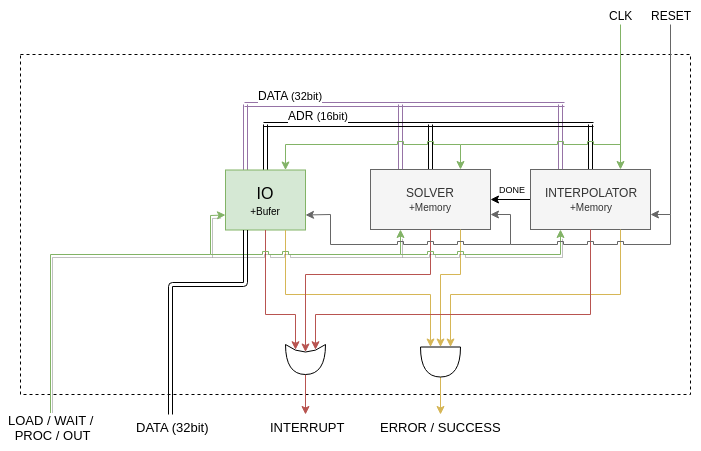
\includegraphics[width=\textwidth]{d1}
    \caption{Overall Design}
    \label{fig:overall}
\end{figure}

\section{Interfaces and HW Summary}
The hardware has the following interfaces that triggers some actions summarized below and detailed in the rest of the document.
\begin{itemize}
    \item CLK: IN
    \item RESET: ASYNC IN
    \begin{itemize}
        \item clears all internal states of all modules:
        \begin{itemize}
            \item IO internal buffer.
            \item ERROR/SUCCESS of all modules resets to SUCCESS.
            \item INTERRUPT resets to zero.
        \end{itemize}
        \item Memory at solver and interpolator are NOT cleared.
        \item at next clock, CPU is expected to turn the \emph{LOAD / WAIT / PROC / OUT} into \emph{LOAD} state and we will start loading input again.
    \end{itemize}
    \item LOAD / WAIT / PROC / OUT (2bit): IN:
    \begin{itemize}
        \item set the current major state of the machine
        \item LOAD(0):
        \begin{itemize}
            \item IO receives \textbf{compressed} data from the CPU.
            \item IO decompresses data into buffer.
            \item buffer is flushed into data bus with appropriate address.
            \item ends when cpu finishes its data loading and switches to \emph{WAIT} state.
        \end{itemize}
        \item WAIT(1):
        \begin{itemize}
            \item Same state as \emph{LOAD}, but IO doesn't receive anymore data from CPU.
            \item ends when IO flushes all its buffer and raises \emph{INTERRUP} with either \emph{ERROR} or \emph{SUCCESS}.
        \end{itemize}
        \item PROC(2):
        \begin{itemize}
            \item SOLVER sends time step to calculate \emph{U} at.
            \item SOLVER and INTERPOLATOR work concurrently to calculate their outputs.
            \item INTERPOLATOR sends \emph{DONE} signal to SOLVER when it finishes the interpolated U.
            \item SOLVER can request to copy the interpolated \emph{U}.
            \item INTERPOLATOR waits for SOLVER to send next time step.
            \item ends when either SOLVER or INTERP raises INTERRUPT with either \emph{SUCCESS} or \emph{ERROR}.
        \end{itemize}
        \item OUT(3):
        \begin{itemize}
            \item IO just copies final outputs to cpu from SOLVER memory.
            \item ends when IO raises INTERRUPT with either \emph{SUCCESS} or \emph{ERROR}.
        \end{itemize}
    \end{itemize}
    \item DATA (32bit): INOUT
    \begin{itemize}
        \item Data bus between cpu and io.
    \end{itemize}
    \item INTERRUPT: OUT
    \begin{itemize}
        \item raised from 0 to 1 when some internal module (IO / SOLVER / INTERPOLATOR) finishes its task.
        \item if task finished with success the \emph{ERROR / SUCCESS} is set to \emph{SUCCESS}, otherwise it's \emph{ERROR}.
    \end{itemize}
    \item ERROR(0) / SUCCESS(1): OUT
    \begin{itemize}
        \item CPU should operate on this value ONLY when \emph{INTERRUPT} is 1.
        \item errors that could happen include: divide by zero, H > 1, incomplete input.
    \end{itemize}
\end{itemize}

\end{document}